\documentclass[portrait,final,a0paper,fontscale=0.32]{baposter}

%%% Basic packages   %%%
\usepackage{calc}
\usepackage{graphicx}
\usepackage{amsmath}
\usepackage{amssymb}
\usepackage{relsize}
\usepackage{multirow}
\usepackage{multicol}
\usepackage{rotating}
\usepackage{bm}
\usepackage{url}
\usepackage{caption}
\usepackage{colortbl}
\usepackage{tabularx}
\usepackage{enumitem}
\usepackage{lipsum}

%%%% Font settings %%%%
\usepackage[mathlf, textlf]{MinionPro}
\usepackage{MyriadPro}
\renewcommand\familydefault{\sfdefault}
\renewcommand{\captionfont}{\footnotesize}

%% Graphics path %%%
\graphicspath{{figs/}{img/}}

%%%% Some math symbols used in the text %%%%
\newcommand{\notes}[1]{\textcolor{red}{#1}}

%%%% Multicol Settings  %%%%
\setlength{\columnsep}{1.5em}
\setlength{\columnseprule}{1mm}

%%%% Save space in lists. Use this after the opening of the list %%%%
\newcommand{\compresslist}{%
\setlength{\itemsep}{1pt}%
\setlength{\parskip}{0pt}%
\setlength{\parsep}{0pt}%
}

%%% Begin Document %%%
\begin{document}
%%% Here starts the poster
%%% Format it to your taste with the options
%%% Define some colors

%\definecolor{lightblue}{cmyk}{0.83,0.24,0,0.12}
\definecolor{pale}{cmyk}{0.16,0.06,0.01,0}
\definecolor{lightblue}{rgb}{0.145,0.6666,1}


\hyphenation{resolution occlusions}
%%%
\begin{poster}%
  % Poster Options
  {
  % Show grid to help with alignment
  grid=false,
  % Column spacing
  colspacing=2em,
  % Number of columns
  columns=2,
  % Color style
  bgColorOne=pale,
  bgColorTwo=lightblue,
  borderColor=blue,
  headerColorOne=blue,
  headerColorTwo=pale,
  headerFontColor=white,
  boxColorOne=white,
  boxColorTwo=lightblue,
  % Format of textbox
  textborder=rounded,
  % Format of text header
  eyecatcher=true,
  headerborder=closed,
  headerheight=0.15\textheight,
%  textfont=\sc, An example of changing the text font
  headershape=rounded,
  headershade=plain,
  headerfont=\Large\textsc, %Sans Serif
  textfont={\setlength{\parindent}{0em}},
  boxshade=plain,
  %background=shade-tb,
  background=plain,
  linewidth=3pt
  }
  % Eye Catcher
  { } 
  % Title
  {\begin{flushleft}
      \textcolor{blue}{\textnormal{\Huge Learning to Identify Diseases From Healthy Medical Images}} \\
      \textnormal{\large Sue Liu, Boris Mitrovic}\\\vspace{-2mm}
      \textcolor{blue}{\textnormal{\large\textbf{Mudano Ltd., UK.}}}\\\vspace{-3mm}
      \textnormal{\normalsize Correspondence to: \textbf{sue.liu@mudano.com}}\vspace{-10mm}
    \end{flushleft}
          
\includegraphics[height=0.0em]{img/mudano_logo}}
            % Authors
     
  % University logo
  {% The makebox allows the title to flow into the logo, this is a hack because of the L shaped logo.
     
\includegraphics[height=3em]{img/mudano_logo}
 
 }
%%%%%%%%%%%%%%%%%%%%%%%%%%%%%%%%%%%%%%%%%%%%%%%%%%%%%%%
%%% Now define the boxes that make up the poster
%%%%%%%%%%%%%%%%%%%%%%%%%%%%%%%%%%%%%%%%%%%%%%%%%%%%%%%
%%% Each box has a name and can be placed absolutely or relatively.
%%% The only inconvenience is that you can only specify a relative position 
%%% towards an already declared box. So if you have a box attached to the 
%%% bottom, one to the top and a third one which should be in between, you 
%%% have to specify the top and bottom boxes before you specify the middle 
%%% box.
%%%%%%%%%%%%%%%%%%%%%%%%%%%%%%%%%%%%%%%%%%%%%%%%%%%%%%%%%%%%%%%
%
% A coloured circle useful as a bullet with an adjustably strong filling

%%%%%%%%%%%%%%%%%%%%%%%%%%%%%%%%%%%%%%%%%%%%%%%%%%%%%%%%%%%%%%%%
\headerbox{Introduction}{name=motivation,column=0,row=0}{
%%%%%%%%%%%%%%%%%%%%%%%%%%%%%%%%%%%%%%%%%%%%%%%%%%%%%%%%%%%%%%%%
  \begin{center}
  \small
    \begin{minipage}{0.96\textwidth}
One major unsolved problem in the field of machine learning is the ability to learning efficiently from few data points, as humans are able to do. Generative models, a branch of unsupervised learning, try to overcome this limitation by learning meaningful features of the input while requiring little or no human supervision or labelling. In the case of disease detection from medical images, by only observing healthy data a generative model will able to identify anomalies for multiple diseases or even rare diseases. This can save time and money in data collection and labelling required for supervised learning methods.
    \vspace{2mm}  
    \end{minipage}

  \end{center}
}
%

    %%%%%%%%%%%%%%%%%%%%%%%%%%%%%%%%%%%%%%%%%%%%%%%%%%%%%%%%%%%%%%%%%%%%%%%%%%%%%%
  \headerbox{Problem}{name=method,column=0,below=motivation}{

%%%%%%%%%%%%%%%%%%%%%%%%%%%%%%%%%%%%%%%%%%%%%%%%%%%%%%%%%%%%%%%%%%%%%%%%%%%%%%
  \small
    \begin{center}
    \begin{minipage}{0.95\textwidth}
    In this study we investigate the problem of unsupervised anomaly detection for retinal diseases. We used an optical coherence tomography OCT dataset [1] containing images of three types of retinal diseases and a set of healthy images.

    \vspace{3mm}
    \end{minipage}

     \begin{minipage}{0.95\textwidth}
     \begin{tabular}{cccc}
     CNV & DME & Drusen & Normal \\
     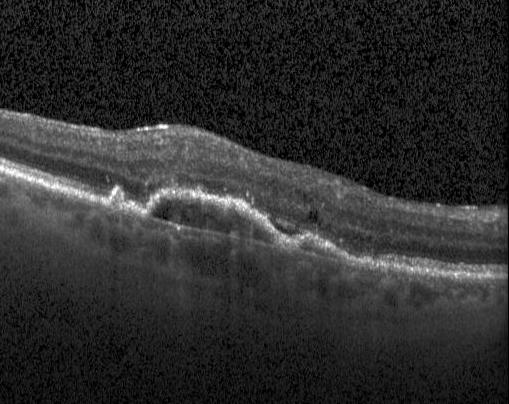
\includegraphics[height=0.15\textwidth]{img/cnv} &
     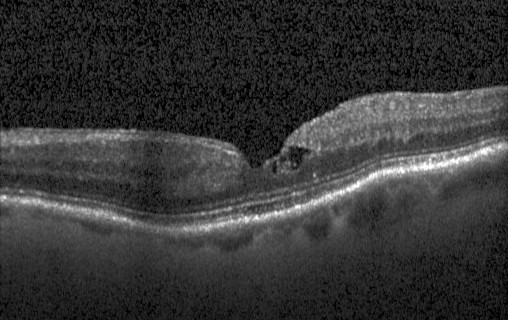
\includegraphics[height=0.15\textwidth]{img/dme} &
     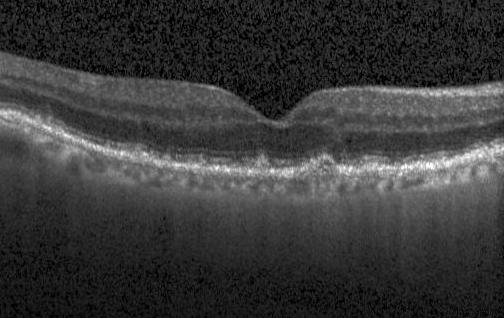
\includegraphics[height=0.15\textwidth]{img/drusen} &
     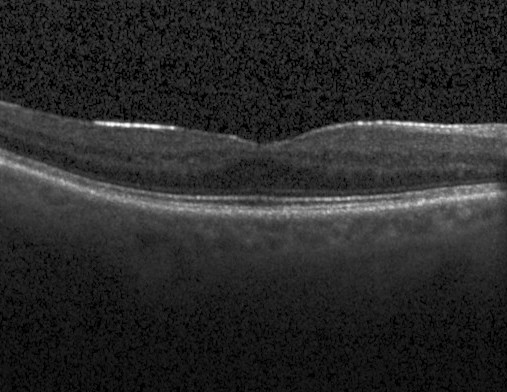
\includegraphics[height=0.15\textwidth]{img/normal} 
     \end{tabular}

     \textit{From left to right:} Choroidal neovascularization (CNV), diabetic macular edema (DME), drusen and normal images. CNV and DME left untreated can result in total blindness, and once diagnosed are immediately referred for treatment. 
     A total of 25236 normal images were used in training and 1329 for validation. The test set consists of 500 images, of which 300 are diseased images and 200 are normal images. 
     \vspace{2mm}
     \end{minipage}
    
\end{center}
}
  %%%%%%%%%%%%%%%%%%%%%%%%%%%%%%%%%%%%%%%%%%%%%%%%%%%%%%%%%%%%%
 \headerbox{Model}{name=dis,column=0,span=1,below=method}{
   %%%%%%%%%%%%%%%%%%%%%%%%%%%%%%%%%%%%%%%%%%%%%%%%%%%%%%%%%%%
   \small
\begin{center}
\begin{minipage}{0.95\linewidth}
 Performing unsupervised learning over images is challenging due to the curse of dimensionality, but the recent development of deep generative models have addressed this issue. One such model is the Variational Autoencoder (VAE) [2, 3].  
\end{minipage}
\small
\begin{minipage}{0.95\textwidth}
\begin{center}
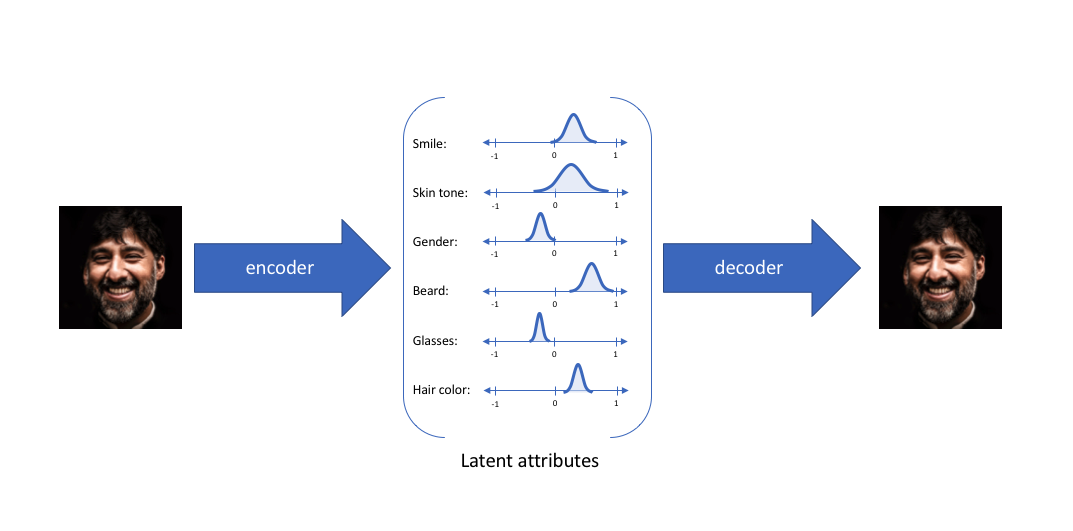
\includegraphics[width=0.75\textwidth]{img/vae_face}

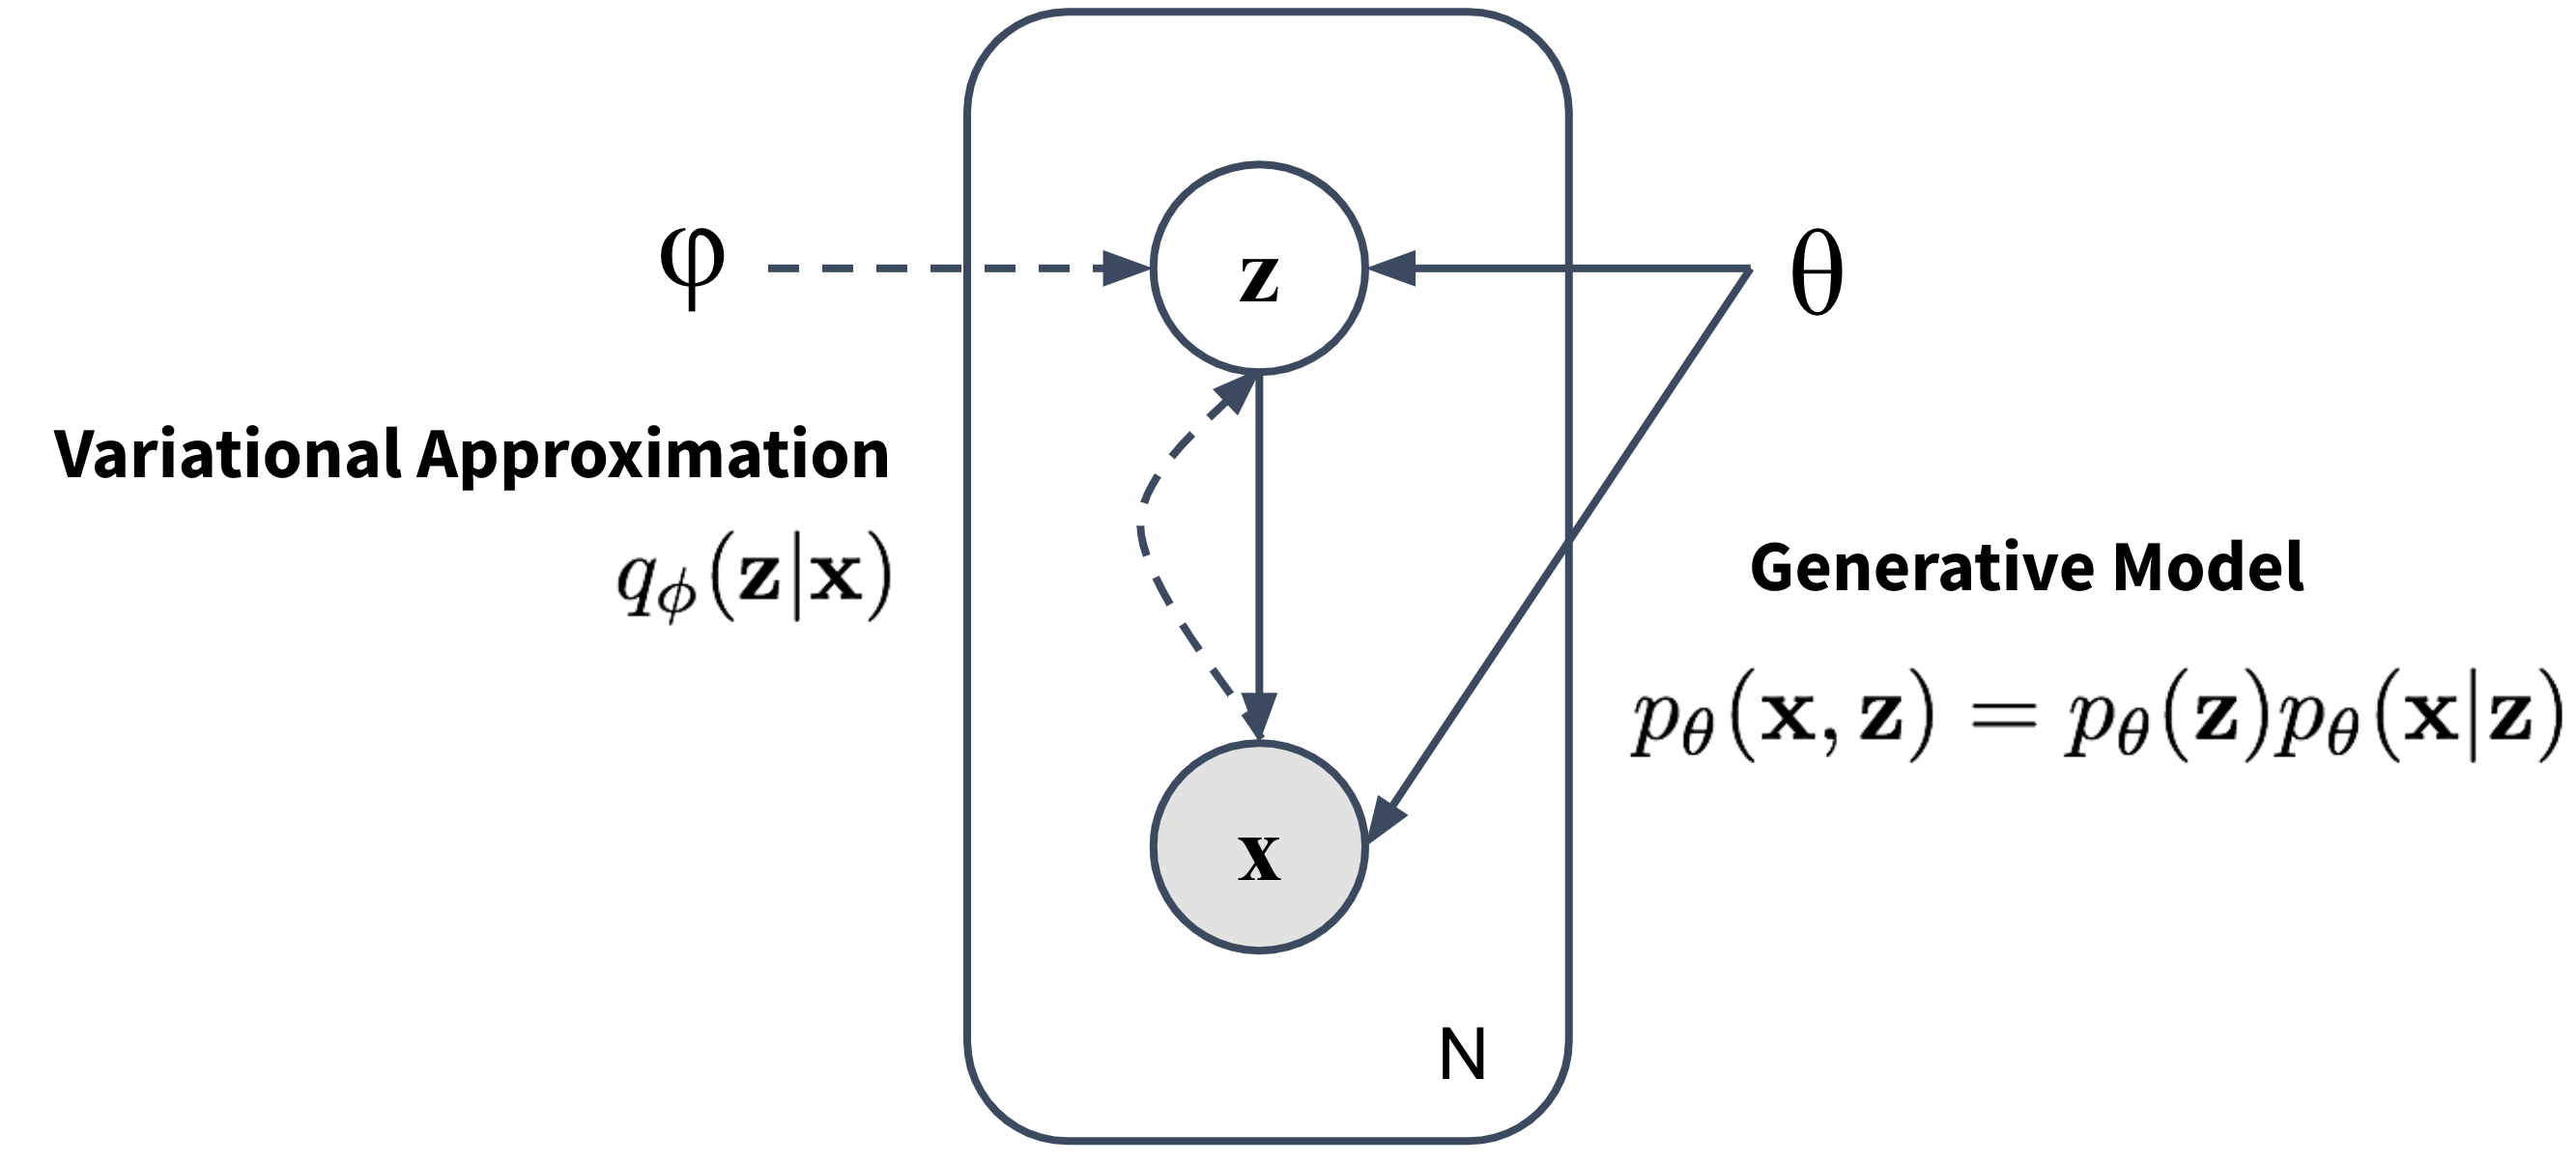
\includegraphics[width=0.57\textwidth]{img/vae_graphical}
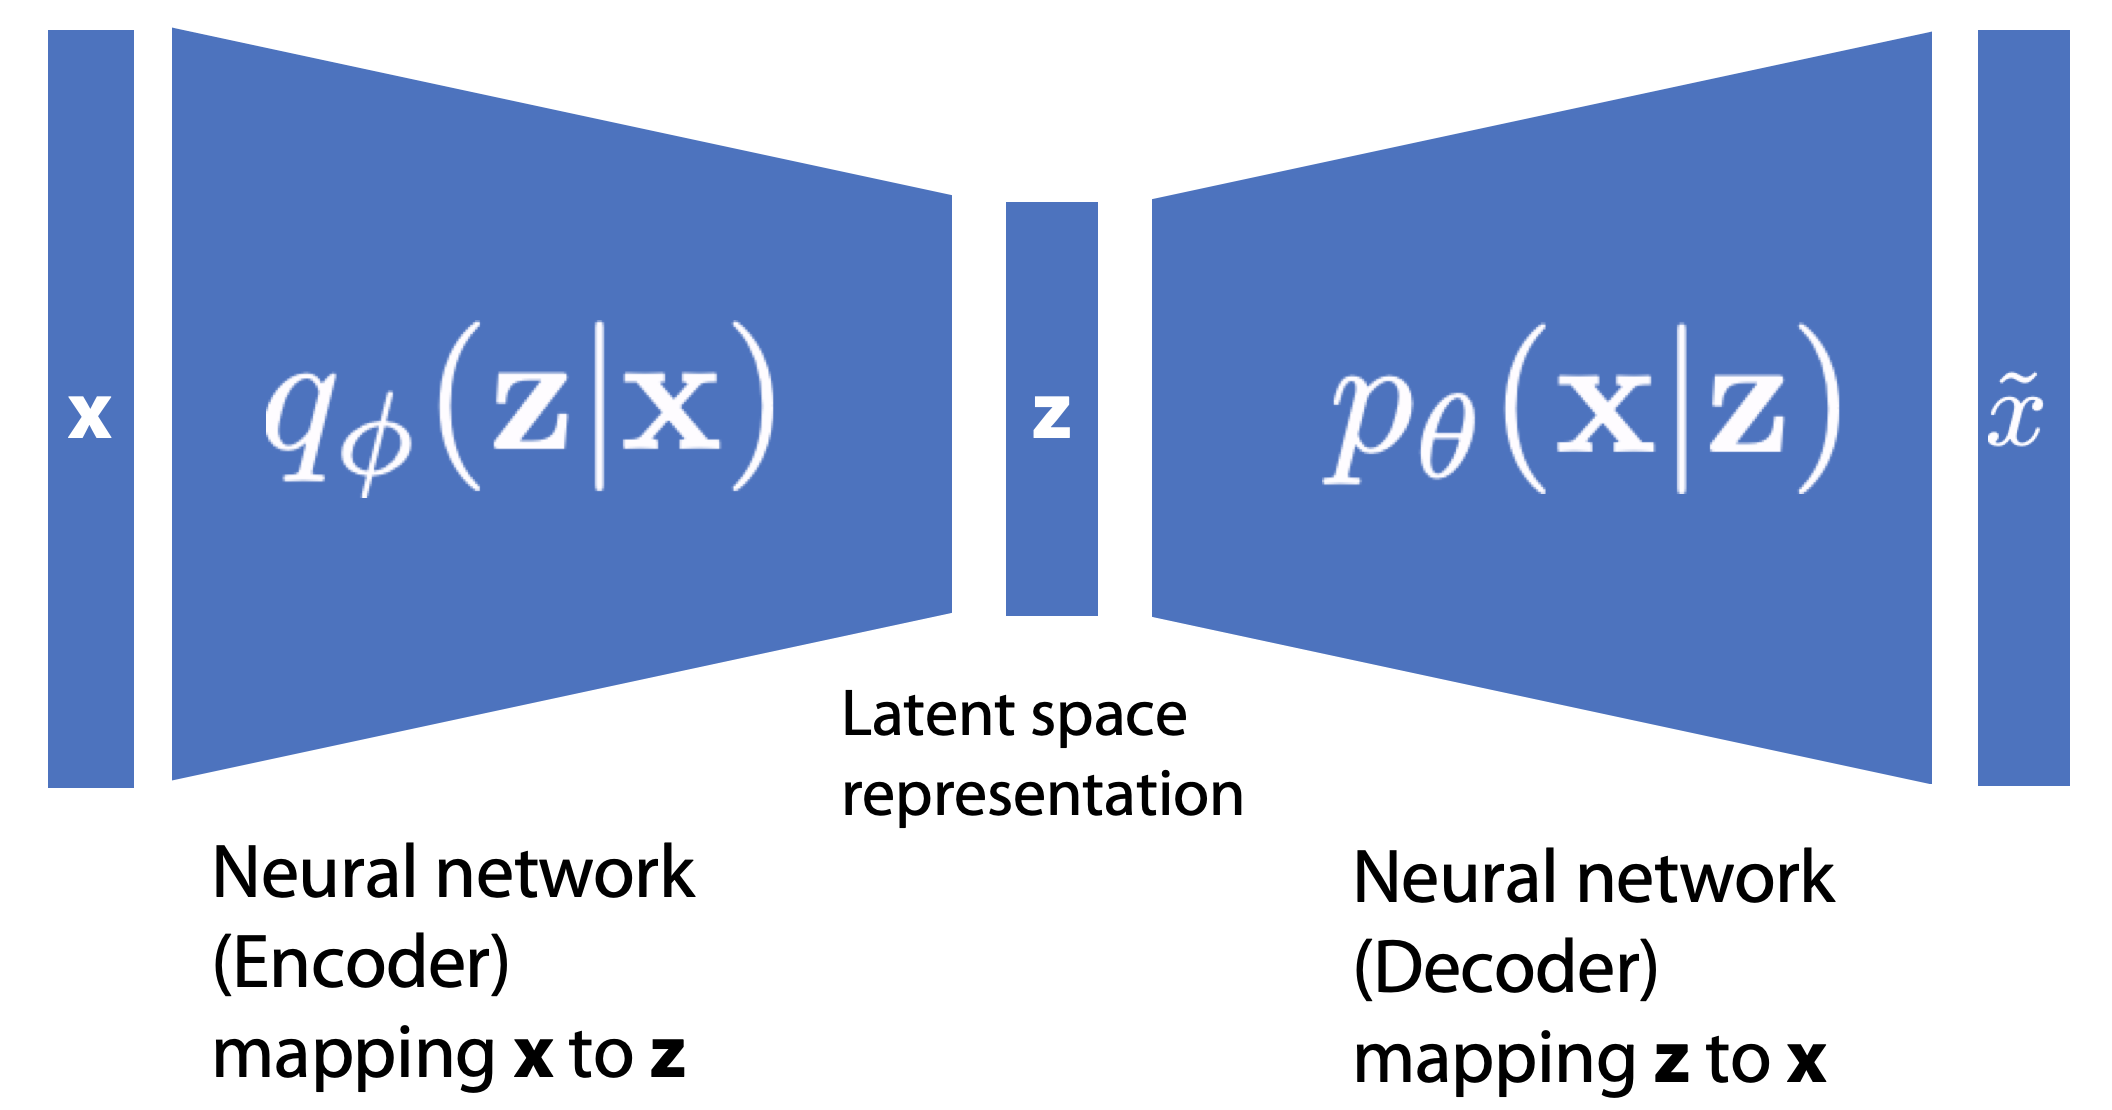
\includegraphics[width=0.37\textwidth]{img/encoder_decoder}
\end{center}
VAE can be viewed as a directed probabilistic graphical model that is constructed into a neural network architecture. The encoder is trained to learn a probabilitic distribution for each latent variable $\mathbf{z}$ from the input $\mathbf{x}$, and the decoder samples the latent distribution $\mathbf{z}$ and learn the mapping $p(\mathbf{x}|\mathbf{z})$ to reconstruct $\mathbf{x}$.

\vspace{1mm}
The learning is performed using variational inference by approximating the conditional distribution $p(\mathbf{z}|\mathbf{x})$ (usually intractable) that describes the mapping from the input to the latent variables by a variational approximation $q(\mathbf{z}|\mathbf{x})$ (defined to have a tractable distribution, usually Gaussian), and maximising the evidence lower bound (ELBO):
$$
\log p(\mathbf{x}) \ge E_{q(\mathbf{z}|\mathbf{x})}\log p(\mathbf{x}|\mathbf{z}) - KL(q(\mathbf{z}|\mathbf{x})||p(\mathbf{z}))
$$
The first term represents the reconstruction likelihood and the second term ensures that our learned distribution $q$ is similar to the true prior distribution $p$.
\vspace{2mm}
\end{minipage}
\end{center}

 }

%%%%%%%%%%%%%%%%%%%%%%%%%%%%%%%%%%%%%%%%%%%%%%%%%%%%%%%%%%%%%%%
  \headerbox{Method}{name=ref,column=0,span=1,below=dis,above=bottom}{
    %%%%%%%%%%%%%%%%%%%%%%%%%%%%%%%%%%%%%%%%%%%%%%%%%%%%%%%%%%%%%%%
    \small
    \begin{center}
    \begin{minipage}{0.95\linewidth}
     We use a fully convolutional architecture similar to that of DCGAN [4]. In the encoder, instead of using a linear layer to produce mean and log variance we use two separate convolutional layers. In this set up the images are normalized to have size 128 x 128, so the encoder consists of 5 convolutional blocks and the decoder consists of 5 deconvolutional blocks. The number of latent dimensions is 300, and the model was trained for 40 epochs using a learning rate of 10$^{-4}$ and ADAM optimizer. 
     \end{minipage}
    \end{center}

   
    }
 

%%%%%%%%%%%%%%%%%%%%%%%%%%%%%%%%%%%%%%%%%%%%%%%%%%%%%%%%%%%%%%%%
  \headerbox{Results}{name=obs,column=1,row=0,span=1}{
    %%%%%%%%%%%%%%%%%%%%%%%%%%%%%%%%%%%%%%%%%%%%%%%%%%%%%%%%%%%%%%%%
    \small
    \begin{center}
    \begin{minipage}{0.95\textwidth}
    \begin{tabular}{cc}
    Original & VAE Generated \\
    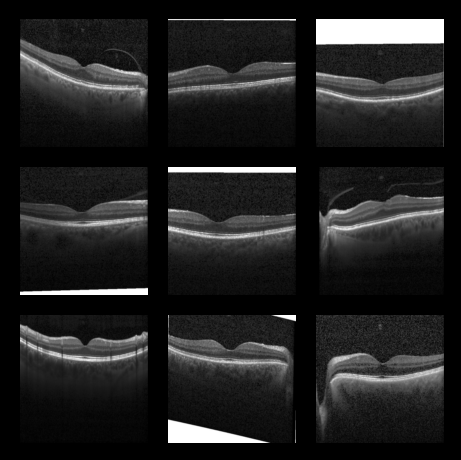
\includegraphics[width=0.48\linewidth]{img/original} &
    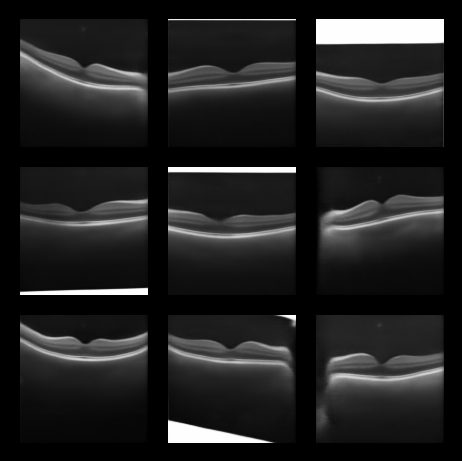
\includegraphics[width=0.48\linewidth]{img/VAE_gen}
    \end{tabular}
    \textit{Above}: 9 randomly selected reconstructions on the validation set. \textit{left:} original images, \textit{right:} VAE reconstructed images. Note that while reconstruction using VAE has captured the significant features in the images, it has smoothed out the edges. This is typical of VAE and pixel based loss function. 
    \vspace{2mm}
    \end{minipage}   
    
    \begin{minipage}{0.95\linewidth}
    \begin{flushleft}
    The degree of anomaly can be characterised by the possibility of seeing $\mathbf{x}$ appear under the distribution $p(\mathbf{x})$, hence computing the anomaly score is essentially estimating $s(\mathbf{x}) = -\log p(\mathbf{x})$, i.e.~the negative of the ELBO loss:
    \end{flushleft}
    
     $$
     s_{\mathbf{VAE}} = KL(q(\mathbf{z}|\mathbf{x})||p(\mathbf{z})) - \frac{1}{L}\sum_{i=1}^L\log p(\mathbf{x}|\mathbf{z}_i), \,\,\,\,\mathbf{z}_i\sim q(\mathbf{z}|\mathbf{x})
     $$
     The first term is the KL-divergence loss and the second the reconstruction loss. 
    \vspace{2mm}
     \end{minipage}

    \begin{minipage}{0.95\linewidth}
    \begin{center}
    \begin{tabular}{r|c|c|c|c}
    
    \textbf{Method used to compute AUC} & \textbf{CNV} & \textbf{DME} & \textbf{Drusen} & \textbf{All} \\
    \hline
    \textbf{Reconstruction Score} & 0.93 & 0.90 & 0.77 & 0.87 \\
    \hline
    \textbf{KL Score} & 0.56 & 0.51 & 0.48 & 0.52 \\
    \hline
    \textbf{VAE Score} & 0.92 & 0.89 & 0.76 & 0.86  
    \end{tabular} 
    \end{center}
    \textit{Table}: AUC values for detecting the three different types of retinal diseases separately and for all diseases. The values are computed using three separate anomaly scores based on reconstruction loss, KL-divergence loss and ELBO loss respectively.
    AUC values obtained using only KL-divergence loss are low, suggesting our prior is not expressive enough to approximate the true latent space distribution.
    \vspace{2mm}
    \end{minipage}
    
    \end{center} 
  }
 
 %%%%%%%%%%%%%%%%%%%%%%%%%%%%%%%%%%%%%%%%%%%%%%%%%%%%%%%%%%%%%%%%%%%%%%%%%%%%%%
  \headerbox{Summary}{name=con,column=1,span=1, below=obs}{
    %%%%%%%%%%%%%%%%%%%%%%%%%%%%%%%%%%%%%%%%%%%%%%%%%%%%%%%%%%%%%%%%%%%%%%%%%%%%%%
    \small
    \begin{center}

    \begin{minipage}{0.95\textwidth}
    \vspace{1mm}
      In this work we have demonstrated the potential of applying Variational Autoencoder (VAE) for anomaly detection in retinal disease images. When trained on only the normal data, the model is able to perform efficient inference and to determine whether a test image is diseased or not. Using the optical coherence tomography (OCT) images from [1], the model is able to detect all diseases with AUC of 0.87, and is able to detect age related macular degeneration and diabetic macular edema, which are diseases requiring immediate referral with AUC of 0.93 and 0.9 respectively. 
      \vspace{1mm}

      VAEs are appealing because they have a solid and elegant theoretical framework, are built on top of standard function approximators (neural networks) and can be easily trained using stochastic gradient descent. In this work we have not fully explored the powers of VAE for anomaly detection: we could perform postprocessing on the anomaly scores and/or make use of the latent space (e.g. create distance metrics).

      \vspace{1mm}
      We argue that although supervised deep learning models have been successfully applied for retinal disease diagnosis [1], applying deep unsupervised learning in disease identification is a promising research direction when the normal images are in abundance, whilst labelled diseases are rare.
    \vspace{3mm}
    \end{minipage}
    \end{center}
}
%%%%%%%%%%%%%%%%%%%%%%%%%%%%%%%%%%%%%%%%%%%%%%%%%%%%%%%%%%%%%
\headerbox{References}{name=end, column=1, span=1,  below=con}{
  \footnotesize
  \bibliographystyle{ieee}
  \renewcommand{\section}[2]{\vskip 0.05em}
  \begin{thebibliography}{1}\itemsep=-0.01em
    \setlength{\baselineskip}{0.4em}
  \bibitem{kermany18}
    D.~S.~Kermany \textit{et al.}
    \newblock Identifying medical diagnoses and treatable diseases by image-based deep learning
    \newblock {\em Cell.}, Vol.172, 2018.
  \bibitem{kingma13}
  D.~P.~Kingma and Welling,~M.
  \newblock Auto-encoding variational Bayes.\\
  \newblock In {\em Proceedings of the 2nd International Conference on Learning Representations}, 2013.
  \bibitem{Rezende14}
  D.~J.~Rezende \textit{et al.}
  \newblock Stochastic backpropagation and approximate inference in deep generative models. 
  \newblock In {\em Proceedings of the 32nd International Conference on Machine Learning (ICML-14)}, 2014. 
  \bibitem{radford2015}
  A.~Radford \textit{et al.}
  \newblock Unsupervised representation learning with deep convolutional generative adversarial networks.
  \newblock In {\em Proceedings of the 5th International Conference on Learning Representations}, 2016.
       \end{thebibliography}
    \vspace{0.3em}
  
}


 %%%%%%%%%%%%%%%%%%%%%%%%%%%%%%%%%%%%%%%%%%%%%%%%%%%%%%%%%%%%%%%%%%%%%%%%%%%%%%
  \headerbox{Acknowledgements}{name=ack,column=1,span=1, below=end, above=bottom}{
    %%%%%%%%%%%%%%%%%%%%%%%%%%%%%%%%%%%%%%%%%%%%%%%%%%%%%%%%%%%%%%%%%%%%%%%%%%%%%%
\small
The authors thank A.~Grivas, J.~Langr and E.~Wielewski for helpful discussions.
    }



\end{poster}

\end{document}
